\documentclass[a4paper]{article}     
\usepackage{amsfonts}
\usepackage{amsmath}
\usepackage{amssymb}
\usepackage{graphicx}
\usepackage{cancel}

\begin{document}
\noindent \large Auteur: Luko De Vriendt\\
\noindent \large Studierichting: Informatica\\
\noindent \large Oefeningenreeks 5G nr. 1.7\\

\medskip

\normalsize

$V = \pi \displaystyle \int_{-\pi}^\pi \cos^2\left(\dfrac{x}{2}\right)dx$ \\

$= \dfrac{\pi}{2}\displaystyle \int_{-\pi}^\pi 1+\cos(x)dx$ \\

$= \dfrac{\pi}{2}\left[x + \sin(x)\right]_{-\pi}^\pi$ \\

$= \dfrac{\pi}{2}((\pi+0)-(-\pi+0))$ \\

$= \pi^2$ \\

\begin{figure}[h]
\centering
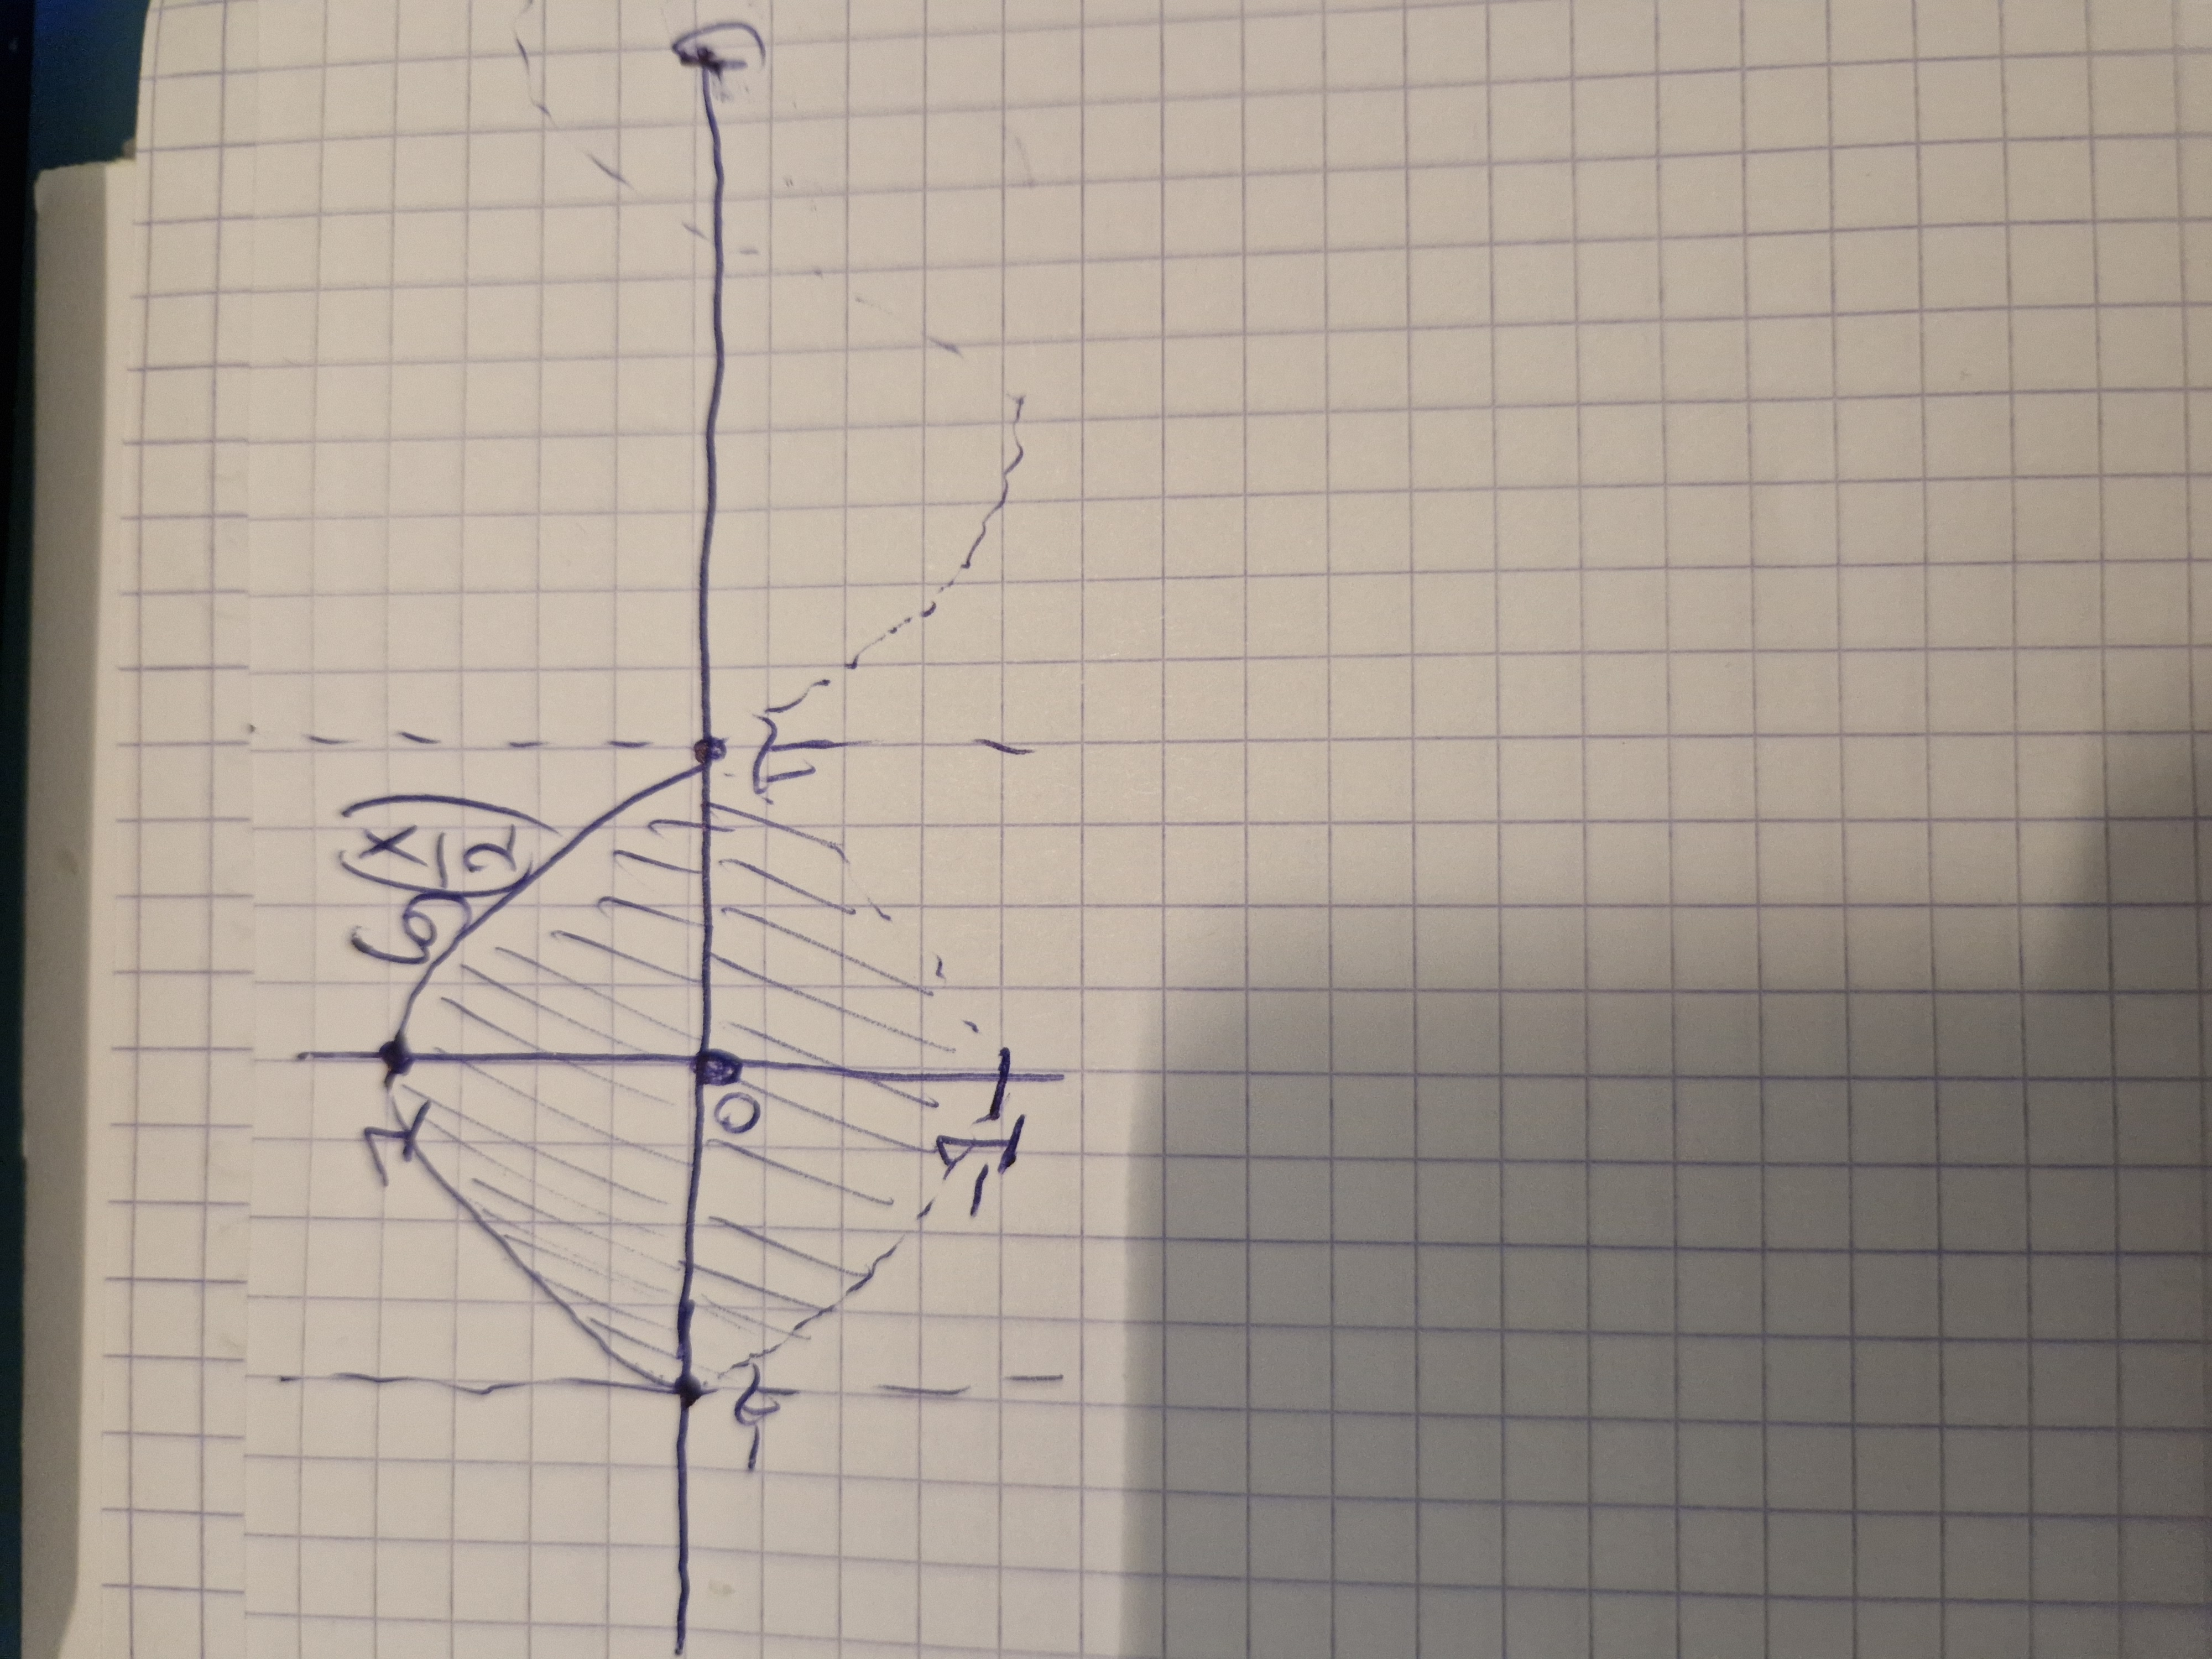
\includegraphics[angle=270,width=10cm]{5G-1.7-luko.de.vriendt.INF.jpg}
\end{figure}

\begin{thebibliography}{999}
%\bibitem{a} Referentie
\end{thebibliography}
\end{document} 
